\documentclass[11pt]{article}
\usepackage[a4paper,margin=24mm]{geometry}
\usepackage[T1]{fontenc}
\usepackage[utf8]{inputenc}
\usepackage{lmodern,microtype,amsmath,amssymb,graphicx,booktabs}
\usepackage[numbers,sort&compress]{natbib}
\usepackage[colorlinks=true,allcolors=blue]{hyperref}
\usepackage{caption}
\usepackage[section]{placeins}
\captionsetup{font=small,labelfont=bf}
\setlength{\parskip}{4pt}
\setlength{\parindent}{0pt}
\newcommand{\charge}{\ensuremath{e}}
\title{Local Chemical Environments Explain Charge-Definition Disagreement in Metal--Organic Frameworks}
\author{Hosein Alimardani$^{1,\dagger}$, Shayan Abaei$^{2,\dagger}$, and Mehrdad Asgari$^{3,*}$\\[5pt]
\small $^1$Faculty of Engineering, University of Tehran, Tehran, Iran\\
\small $^2$School of Chemical Engineering, University of Tehran, Tehran, Iran\\
\small $^3$Lucy Cavendish College, University of Cambridge, Cambridge CB3 0BU, UK\\
\small $^\dagger$Equal contribution. $^*$Correspondence: ma2000@cam.ac.uk}
\date{}
\begin{document}
\maketitle
\begin{abstract}
Local coordination and linker chemistry can organize differences between partial-charge definitions, but element offsets and nonlinear relations between charge scales can mimic an environment effect. We quantify the chemical contribution for DDEC6, CM5, and Bader charges in 9,171 QMOF structures containing 1,420,532 atoms. Matched predictors add first-shell chemistry and two-hop path composition to a flexible control supplied with the central element and source charge. Local information improves held-out all-atom and nonmetal predictions for all three charge pairs, including a split that blocks identical source MOFkeys or reduced formulas. Under this split, DDEC6--Bader structure-balanced mean absolute error decreases from 0.08454 to 0.03885~\charge. A paired chemical atlas shows that directional shifts and greater absolute departures are distinct: O-attached carbon has a DDEC6--Bader signed shift without an established increase in absolute departure, whereas N-attached carbon has a CM5--Bader magnitude increase with a near-zero signed contrast. Central-metal behavior is mixed, including worse DDEC6--Bader prediction after adding structure to the global model. Finite connectivity tests retain the tested nonmetal contrasts while exposing shared-proton ambiguity. The atlas thus identifies conditional chemical structure in charge-definition disagreement, with an explicit distinction between empirical departures and physical charge accuracy.
\end{abstract}
\noindent\textbf{Keywords:} metal--organic frameworks; partial atomic charges; local chemical environments; QMOF; conditional prediction

\section{Introduction}
Local coordination and linker substitution give metal--organic frameworks (MOFs) a chemically diverse electrostatic landscape. Partial atomic charges translate that landscape into parameters used in atomistic simulations, but the assigned values depend on how the electron density is represented. This dependence matters in practice: systematic adsorption calculations show that changing framework point charges can alter carbon dioxide and water isotherms, with particularly strong sensitivity at open metal sites.\cite{Sladekova2020,SladekovaCorrection2021} Understanding how charge definitions respond to local chemistry is therefore useful even when no single definition can serve as a universal reference.

Bader analysis partitions electron density into atomic basins, DDEC6 balances electrostatic and chemical objectives, and CM5 maps Hirshfeld populations through a parameterized charge model.\cite{Tang2009,Manz2016,ManzCorrection2022,Marenich2012} Their differences reflect distinct definitions of an atomic contribution to a continuous density. A signed difference between two assignments consequently describes their relationship; it does not measure an observable charge error. Local environments may organize that relationship by producing directional shifts, larger departures from an average mapping, or a broader range of departures within the same class. These possibilities require separate summaries.

The Quantum MOF (QMOF) Database provides aligned structures and charge assignments for examining these questions at scale.\cite{Rosen2021} Rosen and co-workers already established substantial differences among DDEC6, Bader, and CM5 charges, often exceeding changes associated with the tested density functional approximations.\cite{Rosen2022} Structural charge predictors, including PACMAN, further demonstrate that a specified charge definition can be learned from crystal environments.\cite{Zhao2024,Zhao2024Correction} Neither observation by itself establishes how much chemical information remains in a difference between charge definitions once the central element and one of the charges are known. A structural model can otherwise appear successful by recovering element offsets or curvature between charge scales.

We address this conditional question by comparing matched predictors of an ordered charge difference. A flexible predictor supplied with the element and source charge provides the control; first-shell descriptors and then two-hop path composition provide successive additions. Withholding complete structures tests prediction beyond the fitting records. A second split keeps records with identical source MOFkeys or reduced formulas together, addressing a specified form of related-record dependence. This design makes the chemical contribution assessable without treating prediction error against one charge definition as physical accuracy.

For a common cohort of 9,171 QMOF structures, we combine these comparisons with a paired atlas of chemically interpretable environments. The atlas separates signed departure, absolute departure, and within-environment residual spread. Carbon attachment classes illustrate why these quantities lead to different conclusions, while population-specific evaluation reveals a central-metal failure hidden by the overall improvement. Finite graph tests then delimit the stability of the tested contrasts and identify shared-proton ambiguity. The resulting contribution is a quantitative account of how local chemistry organizes charge-definition disagreement within the evaluated cohort and models.

\section{Methods}
\subsection{Source data and aligned cohort}
Structures and partial charges were taken from the pinned QMOF Figshare release, article 13147324, version 18, archive file 59573735.\cite{Rosen2021,Rosen2022,QMOFv18} No new electronic-structure calculations or experimental measurements were performed. The common finite-charge cohort contains 9,171 structures and 1,420,532 atoms, including 46,994 metal atoms in 9,165 structures. Atomic records were aligned by QMOF identifier and source atom index, with element identity and source site order checked. The common cohort is the intersection of available finite charge assignments, rather than a sample selected for a particular chemical effect. The structural and charge tables and graph configuration \nolinkurl{621045db53a892f1} were fixed before the conditional comparisons.

For an ordered pair of charge definitions $A$ and $B$, the target is
\begin{equation}
 \Delta_i^{AB}=q_i^A-q_i^B.
\end{equation}
We report DDEC6--CM5, DDEC6--Bader, and CM5--Bader in this order. These targets are algebraically dependent, since $\Delta^{\mathrm{DDEC6,Bader}}=\Delta^{\mathrm{DDEC6,CM5}}+\Delta^{\mathrm{CM5,Bader}}$; they are not three independent replications. Neither definition is treated as ground truth.

\subsection{Periodic local environments}
Structures were handled with pymatgen and ASE.\cite{Ong2013,Larsen2017} Metals follow \nolinkurl{pymatgen.core.Element.is_metal}. Nonmetal--nonmetal contacts were accepted between 0.40~\AA\ and 1.25 times the sum of ASE covalent radii. Metal-involving contacts used CrystalNN\cite{Zimmermann2020} without oxidation-state assignments and with electronegativity weighting disabled. A metal--nonmetal edge was accepted when selected by the metal center; a metal--metal edge was accepted when selected by either metal center. Every accepted edge was given an explicit reverse, retaining distinct periodic images of the same indexed neighbor. The complete parameter set and ambiguity definitions are given in the supporting information.

First-shell features describe the composition and distances of the selected neighborhood. Two-hop features count non-backtracking paths through that graph; they do not count unique atoms at graph distance two. Central-element information and the structural feature dictionary were fixed. No target charge, oxidation-state assignment, spin density, or electronic bond order entered graph selection. Diagnostic flags identify potentially ambiguous neighborhoods without declaring them chemically incorrect. Graph construction completed for every structure. The 72 zero-neighbor atoms and all flagged sites were retained.

\subsection{Conditional charge mappings and model comparison}
Within each training fold, an element-specific 12-bin piecewise charge mapping supplied a common prediction of $\Delta^{AB}$ from $q^A$. Training quantile bins, interpolation, endpoint extrapolation, and affine or global fallbacks are specified in the supporting information. Each competitor then predicted the residual to this common mapping. We compared an element residual mean, a flexible tree using central-element information and $q^A$, the same tree with first-shell features added, and the same tree with first-shell and two-hop features. Thus, only the charge-only to first-shell comparison isolates the first-shell contribution conditional on the source charge; the first-shell to two-hop comparison tests path information beyond that first shell. The charge-only to two-hop gain is the principal overall conditional comparison.

All tree fits used XGBoost\cite{Chen2016} with 100 estimators, maximum depth four, learning rate 0.08, minimum child weight 20, and $L_2$ penalty five. The algorithm, feature dictionary, training sample, and weights were matched across competitors. Training was capped at 160,000 atoms per fold through a deterministic structure--element sampling rule, with weights corrected for the retained sample. Every held-out atom was evaluated. No hyperparameter search, early stopping, or held-out model selection was performed. The source charge was permitted only in these explicitly conditional analyses; the target scheme's charge was never a predictor.

\subsection{Structure and identifier/composition validation}
Five original folds withheld entire structures. A second five-fold split linked records into connected components when they shared either a nonempty exact source MOFkey\cite{Bucior2019} or an exact source reduced formula. This created 8,347 components, including 1,414 records in nonsingleton components. Components were assigned intact to folds containing 1,835, 1,834, 1,834, 1,834, and 1,834 structures. All calibrations and residual models were newly fitted for this split. MOFkey-present and nonsingleton records were also evaluated separately. This tests the specified identifier/composition dependence; it does not establish separation of every chemical family or unseen topology.

The principal error is the structure-balanced mean absolute error,
\begin{equation}
 \mathrm{MAE}_{\mathrm{str}}=\frac{1}{N}\sum_{s=1}^{N}
 \frac{1}{n_s}\sum_{i\in s}\left|\Delta_i^{AB}-\widehat{\Delta}_i^{AB}\right|,
\end{equation}
where $n_s$ is the number of evaluated atoms in structure $s$ for the stated population. Atom-weighted errors are reported separately. Positive gain denotes baseline MAE minus structural-model MAE on the same held-out atoms. Intervals use 1,000 paired bootstrap draws over structures for the original folds and over components for the blocked folds. Component resampling retains sums of per-structure losses and structure counts, preserving the structure-balanced estimand. These pointwise intervals condition on the fitted models and do not include uncertainty from retraining or unrecognized broader families.

\subsection{Chemical atlas and graph sensitivity}
For the chemical atlas, the flexible charge-only held-out residual is $r_i=\Delta_i^{AB}-\widehat{\Delta}_{i,\mathrm{charge}}^{AB}$. We separately summarize $\Delta_i^{AB}$, $|\Delta_i^{AB}|$, $r_i$, $|r_i|$, and the within-structure/environment standard deviation of $r_i$. Same-element environment contrasts are paired within structures before averaging. Six fixed contrasts compare O-attached or N-attached carbon with strictly C/H-only carbon, O-bound or N-bound monocoordinate H with C-bound H, and metal-adjacent O or N with their non-metal-adjacent counterparts. N-attached carbon excludes O attachment. Compact atlas entries require at least 30 structures and 30 represented validation units; the full tables retain lower-support classes.

Graph sensitivity used a fixed 96-structure subset containing 16,165 atoms. The nonmetal radius scale was changed to 1.20 and 1.30 while accepted metal-involving edges were held fixed. Descriptors, environment membership, and paired contrasts were recomputed with the same held-out residuals, comparing common paired structures. Separate, earlier fixed-model perturbations of metal contacts are reported with their original model population and conditioning; they are not refits of the conditional models. The graph is an operational environment definition, not a universal chemical bond assignment.

\section{Results and discussion}
\FloatBarrier
\subsection{Charge definitions produce element-dependent differences}
Charge definitions differ in both scale and direction across elements (Figure~\ref{fig:landscape}). The structure-balanced DDEC6--Bader mean is $-0.29096$~\charge\ for carbon and $+0.58916$~\charge\ for oxygen; the corresponding DDEC6--CM5 means are $+0.03938$ and $-0.23530$~\charge. Thus, the sign of an elementwise difference can reverse with the charge pair. These means describe the same aligned atomic sites, but an environment contrast could still reflect different sampling of an element-specific charge relation. The conditional models test what remains after that relation is supplied explicitly.

All three pairs use the same availability-defined cohort. Graph construction completed for all structures, while 24,297 atoms received diagnostic ambiguity flags. Keeping these sites in the atlas preserves the environments where an operational neighborhood assignment deserves closer inspection; it does not equate a flag with an incorrect bond.

\begin{figure}[!htbp]
\centering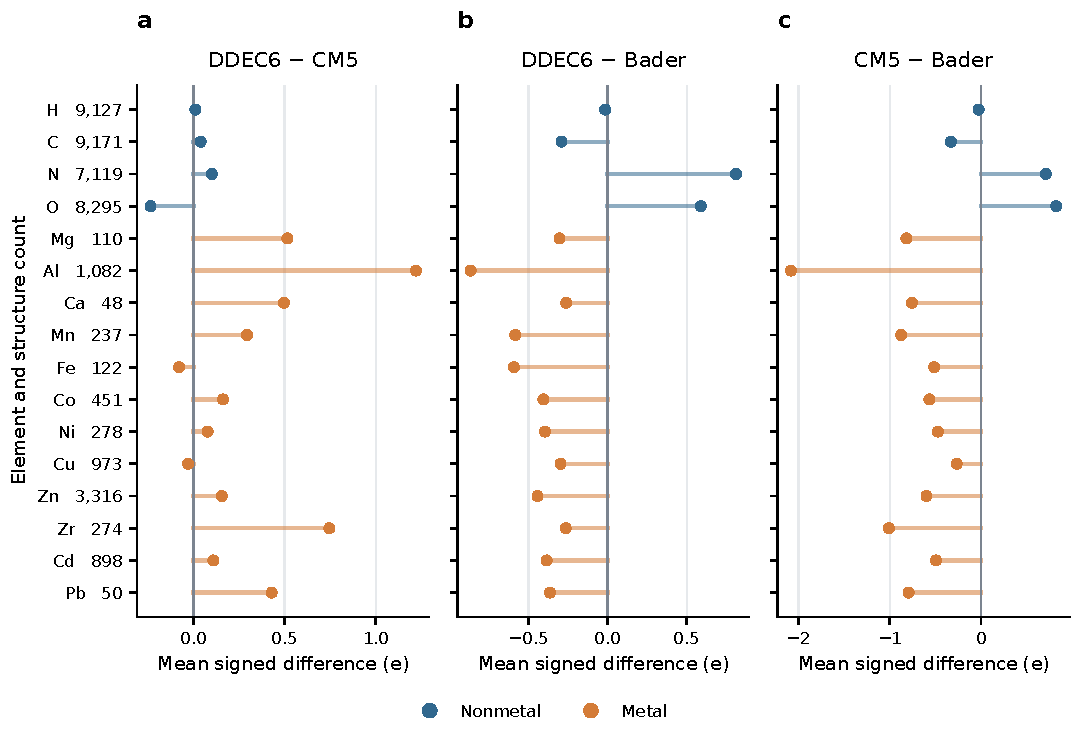
\includegraphics[width=\textwidth]{figures/Figure_01_charge_landscape.pdf}
\caption{\textbf{Element-dependent charge-definition disagreement.} Structure-balanced mean signed differences for 16 displayed elements in the 9,171-structure common cohort. Points are descriptive means; no uncertainty intervals are plotted. Each structure contributes equally within the stated element population. Orange marks metal elements and blue marks nonmetals under the operational classification. Counts beside the elements are numbers of represented structures; the same structure can contribute to multiple elements. Points describe charge definitions and are not errors relative to a reference charge. Complete distributions are retained with the numerical evidence.}
\label{fig:landscape}
\end{figure}

\FloatBarrier
\subsection{Local chemistry contributes beyond the tested charge-only mapping}
Adding local structural information reduces held-out error after a flexible relation between charge definitions has already been fitted (Figure~\ref{fig:conditional}). Under identifier/composition blocking, the charge-only to two-hop MAE decreases are 0.02434 to 0.01018~\charge\ for DDEC6--CM5, 0.08454 to 0.03885~\charge\ for DDEC6--Bader, and 0.06750 to 0.03914~\charge\ for CM5--Bader. Table~\ref{tab:main} reports the matched gains and paired intervals. The gains correspond to approximately 58\%, 54\%, and 42\% of charge-only MAE, respectively. Every all-atom gain is positive in all five folds under both validation schemes (Figure S3).

\begin{table}[!htbp]
\centering\small
\caption{Identifier/composition-blocked structure-balanced MAE and paired two-hop gain over charge only, in e. All 9,171 structures and 1,420,532 atoms are evaluated. Intervals are pointwise 95\% component-bootstrap intervals conditional on fitted models.}
\label{tab:main}
\setlength{\tabcolsep}{3pt}
\begin{tabular}{lrrrrl}
\toprule
Charge pair & Charge only & First shell & Two-hop & Gain & 95\% interval \\
\midrule
DDEC6--CM5 & 0.02434 & 0.01309 & 0.01018 & 0.01416 & [0.01400, 0.01432] \\
DDEC6--Bader & 0.08454 & 0.04197 & 0.03885 & 0.04569 & [0.04495, 0.04640] \\
CM5--Bader & 0.06750 & 0.03981 & 0.03914 & 0.02837 & [0.02782, 0.02893] \\
\bottomrule
\end{tabular}
\end{table}


Most of the reduction comes from the first shell, consistent with immediate chemical context carrying information that the source charge alone does not encode in these regressors. Two-hop paths then reduce blocked MAE by a further 0.00291, 0.00311, and 0.00068~\charge\ for the three ordered pairs, respectively. The smaller path increments indicate information beyond immediate neighbors. This is a comparison of fixed regressors: the gain quantifies the information recovered by these representations and controls, rather than exhausting every possible scalar mapping.

Related-record blocking leaves the principal result intact. The 1,414 records in nonsingleton components retain gains of 0.01306~\charge\ for DDEC6--CM5, 0.04664~\charge\ for DDEC6--Bader, and 0.02687~\charge\ for CM5--Bader, with intervals above zero. The improvement is therefore also present in the subset directly affected by grouping. However, exact formula and MOFkey blocking are conservative operational checks, not proof of transfer to wholly new linkers, metals, or topologies.

\begin{figure}[!htbp]
\centering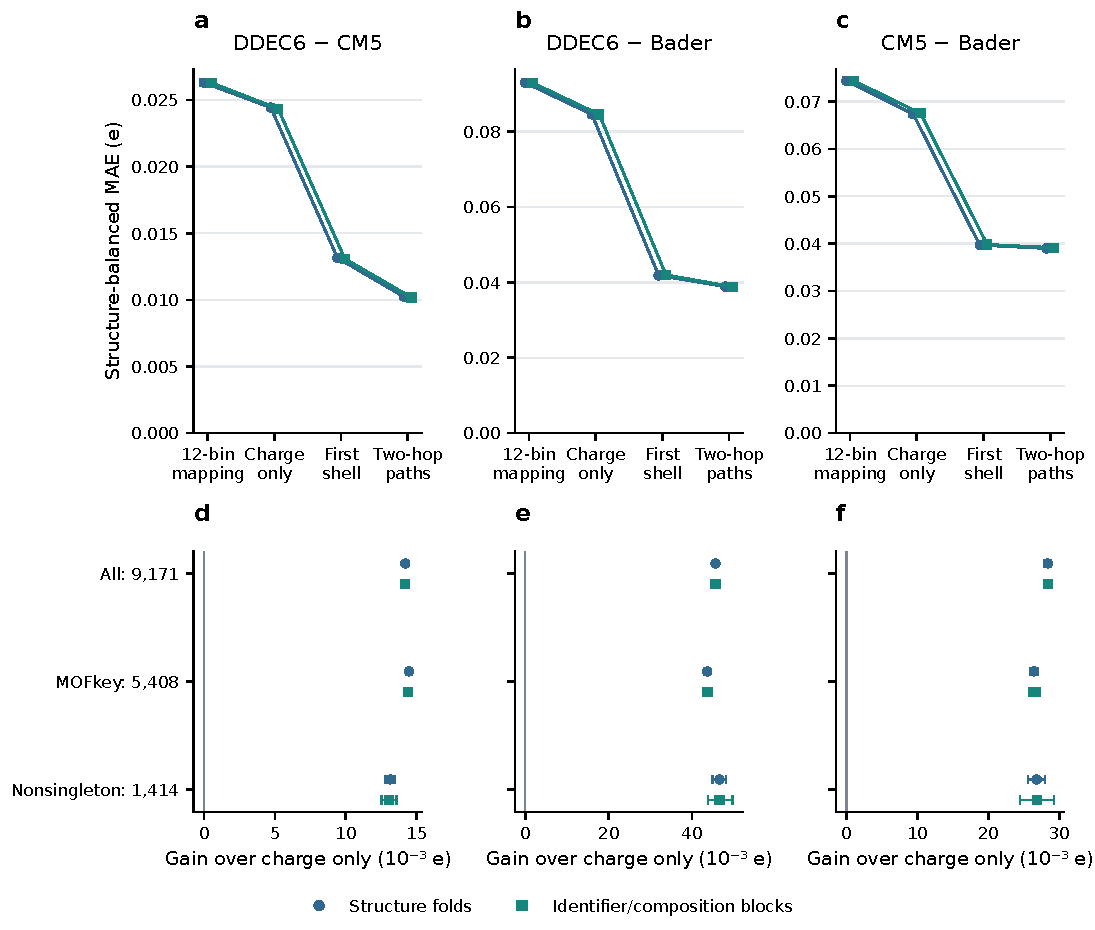
\includegraphics[width=\textwidth]{figures/Figure_02_conditional_evidence.pdf}
\caption{\textbf{Structural information survives charge conditioning and the specified blocking challenge.} (a--c) Structure-balanced held-out MAE for the training-fitted piecewise mapping, flexible charge-only tree, and nested first-shell and two-hop models, over all 9,171 structures and 1,420,532 atoms. All tree competitors share fitting atoms and weights. (d--f) Paired MAE gain of the two-hop model over the flexible charge-only model for all records, MOFkey-present records, and records in nonsingleton blocking components. The panels retain separate charge-pair scales. Error bars are pointwise 95\% bootstrap intervals, resampling structures or identifier/composition components as appropriate. Intervals condition on the fitted models.}
\label{fig:conditional}
\end{figure}

\FloatBarrier
\subsection{Directional shifts and larger departures are different chemical findings}
The environment atlas asks a complementary question: where do charge differences depart from the flexible charge-only relation? Figure~\ref{fig:contrasts} separates paired contrasts in signed residuals from paired contrasts in absolute residuals. Positive and negative signs refer to the fixed ordering $q^A-q^B$ and to the left environment minus the right environment. They are not oxidation-state changes.

O-attached carbon provides a clear distinction. Relative to strictly C/H-only carbon, the blocked DDEC6--Bader signed departure contrast is $-0.07210$~\charge\ (95\% interval $[-0.07491,-0.06946]$; 7,601 paired structures). The corresponding absolute-departure contrast is $-0.00112$~\charge\ with an interval spanning zero, $[-0.00342,0.00126]$. The directional shift therefore does not establish larger absolute disagreement in this contrast.

The converse occurs for N-attached, O-absent carbon in CM5--Bader. Across 6,689 paired structures, its signed contrast against C/H-only carbon is close to zero, $+0.00068$~\charge\ ($[-0.00378,0.00540]$), while its absolute-departure contrast is $+0.10216$~\charge\ ($[0.09904,0.10558]$). Cancellation in a signed summary can therefore coexist with a substantial difference in departure magnitude. The residual-spread contrasts also differ: O-attached carbon has a lower within-environment spread by 0.03488~\charge, whereas N-attached carbon has a higher spread by 0.03716~\charge\ in the respective comparisons. These are differences in averages of within-structure standard deviations, not pooled spreads or uncertainty in a physical charge. Figure S4 places these examples within the broader supported atlas.''

The size of a chemical contrast also depends on the scalar relation removed before constructing the atlas. For example, the original-fold DDEC6--CM5 N--H versus C--H signed contrast changes from approximately $-0.06788$~\charge\ after the earlier piecewise-only correction to $-0.02187$~\charge\ after the flexible charge-only correction. The persistence of a chemical contrast must therefore be evaluated against its stated control, not inferred from an unadjusted comparison. The atlas retains these distinctions, support counts, and ambiguity coverage; the full set includes weak and null contrasts.

\begin{figure}[!htbp]
\centering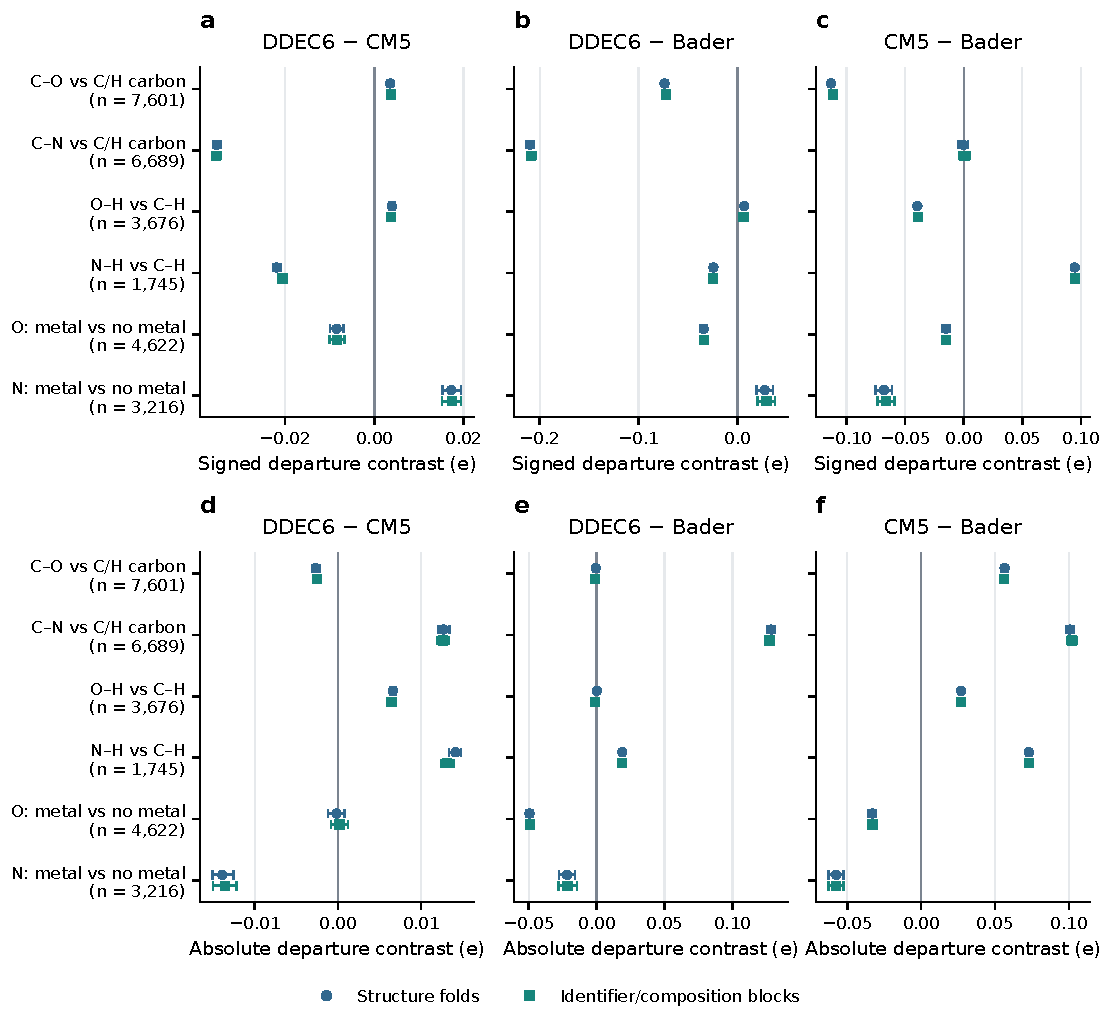
\includegraphics[width=\textwidth]{figures/Figure_03_chemical_contrasts.pdf}
\caption{\textbf{Chemical shifts do not imply larger absolute departures.} Paired within-structure contrasts after subtraction of the flexible charge-only held-out prediction. (a--c) Signed residual contrasts. (d--f) Absolute residual contrasts. Each row compares two environments of the same element within structures containing both classes; $n$ is the number of paired structures. C--N denotes N-attached, O-absent carbon; C/H carbon has only C/H neighbors. H classes require monocoordinate H. Metal adjacency follows the accepted graph. Points show the original and identifier/composition-blocked splits; error bars are pointwise 95\% paired bootstrap intervals, with no multiplicity adjustment. The three pair targets are algebraically related. These descriptive contrasts quantify empirical mapping departures rather than causal effects or physical charge error.}
\label{fig:contrasts}
\end{figure}

\FloatBarrier
\subsection{The all-atom result does not imply a general central-metal benefit}
Metal-centered predictions give a more qualified result (Figure~\ref{fig:metal}). Across 46,994 metal atoms in 9,165 structures, adding local structural features to the global conditional model improves blocked DDEC6--CM5 MAE from approximately 0.02694 to 0.02202~\charge. The gain is 0.00493~\charge\ ($[0.00451,0.00533]$). CM5--Bader shows a much smaller gain, 0.00091~\charge\ ($[0.00049,0.00137]$).

For DDEC6--Bader, the same comparison worsens metal MAE from approximately 0.02044 to 0.02851~\charge. The negative gain, $-0.00807$~\charge\ ($[-0.00857,-0.00749]$), occurs in all five blocked folds. This failure is not removed by the strong all-atom result. A global fitting population can capture the dominant nonmetal pattern while giving a different result at metal centers. Metals constitute only about 3.3\% of the atoms, so aggregate success can coexist with deterioration at their centers. Structure balancing prevents large structures from dominating the metric, but does not make a global training population equivalent to a metal-specific one. The earlier metal-only model is reported separately as a follow-up to a global failure; it does not replace this conditional result.

\begin{figure}[!htbp]
\centering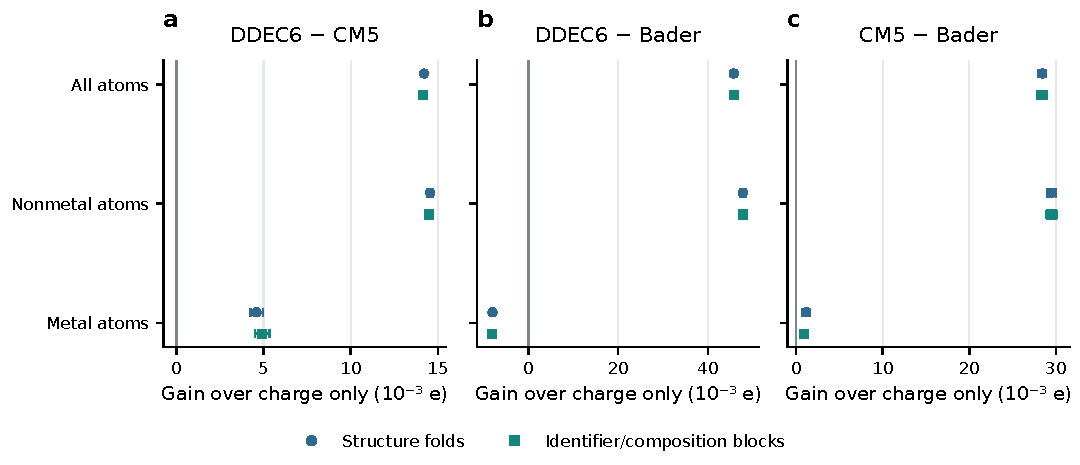
\includegraphics[width=\textwidth]{figures/Figure_04_population_limits.pdf}
\caption{\textbf{Population-specific limits of the conditional result.} MAE gain of the two-hop conditional model over the flexible charge-only model for all atoms, nonmetal atoms, and central metal atoms. Positive values favor the structural model; negative values indicate worse prediction. Original and identifier/composition-blocked fits are shown separately with pointwise 95\% paired bootstrap intervals. The global DDEC6--Bader metal failure is retained. The metal population is 46,994 atoms in 9,165 structures; population means weight represented structures equally. Panels use separate horizontal scales; the small CM5--Bader metal gain should not be equated with the larger all-atom gains.}
\label{fig:metal}
\end{figure}

\FloatBarrier
\subsection{Connectivity uncertainty bounds the chemical interpretation}
The graph determines which local environment is assigned to an atom. Its influence must therefore be distinguished from charge-definition disagreement itself. On the fixed 96-structure subset, lowering the nonmetal radius scale from 1.25 to 1.20 changes no first shells. Raising it to 1.30 adds 12 image-aware, unoriented contacts and changes 18 first-shell and 38 two-hop feature records. The six tested headline environment memberships and their common-pair contrasts remain unchanged on this subset (Figure~\ref{fig:graph}; Figure S5).

The wider cutoff nevertheless exposes a chemically meaningful ambiguity. Six H sites lie close to the midpoint of nearly linear O--H--O arrangements, with added H--O distances of approximately 1.2125--1.2200~\AA. At representative sites, the accepted graph gives isolated H, whereas the wider graph gives two O neighbors. Neither a stable headline contrast nor agreement between graph algorithms adjudicates the physical proton configuration. Such cases remain flagged rather than silently assigned to an ordinary monocoordinate O--H class.

Earlier fixed-model metal-graph perturbations also change prediction errors, especially under a replacement by the original radius-cutoff graph (Figure~\ref{fig:graph}c). These tests use the earlier metal-only model and the same finite subset; they are not perturbation tests of the final conditional fits. Their role is to demonstrate representation dependence and motivate explicit graph scope. The finite nonmetal test supports stability of the listed contrasts on these 96 structures, not universal graph robustness across the whole cohort.

\begin{figure}[!htbp]
\centering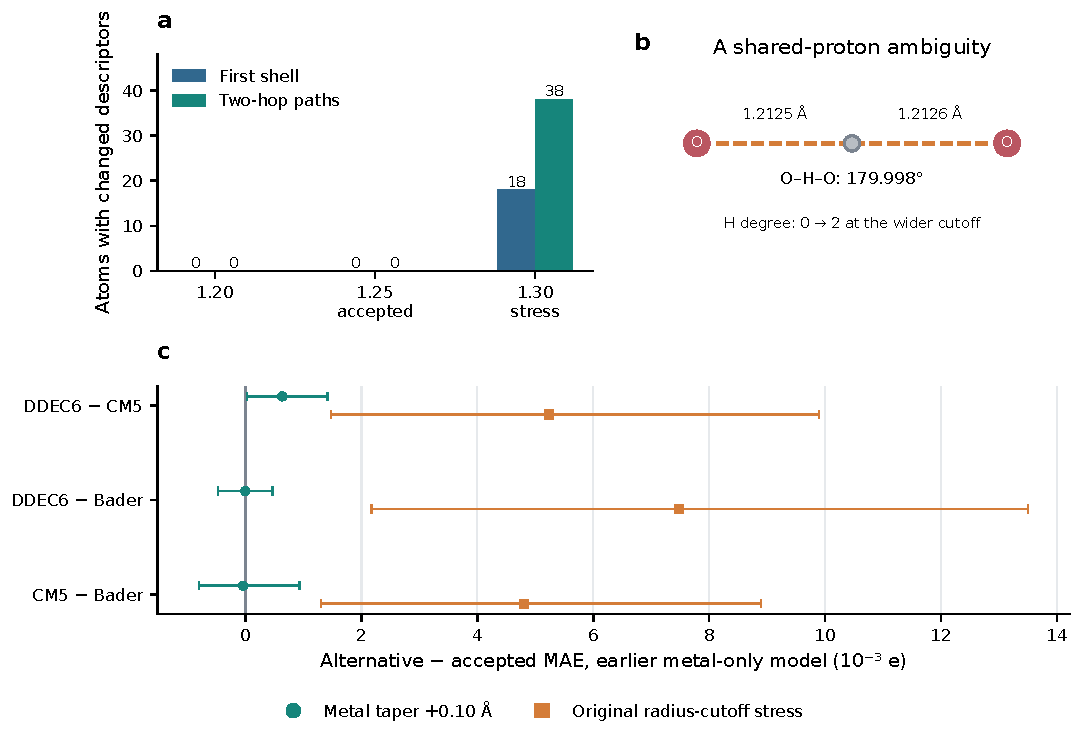
\includegraphics[width=\textwidth]{figures/Figure_05_connectivity_limits.pdf}
\caption{\textbf{Connectivity stability and ambiguity are distinct.} (a) Atoms with changed first-shell or two-hop features under nonmetal cutoff scales 1.20 and 1.30 relative to 1.25, on 96 structures containing 16,165 atoms; metal-involving edges are fixed. (b) One recorded near-midpoint O--H--O geometry, reconstructed from its saved distances and angle. Dashed contacts are added by the wider stress cutoff; the drawing is a local geometry illustration, not a bond-truth assignment. Six H sites exhibit this ambiguity. (c) Earlier fixed metal-only two-hop model sensitivity to a shifted metal distance taper and to the original radius-cutoff stress graph, using 508 metal atoms on the 96-structure subset. Error bars are the saved pointwise 95\% structure-bootstrap intervals. Panel (c) is explicitly an earlier model diagnostic and must not be read as a refit or sensitivity test of the final charge-conditioned models.}
\label{fig:graph}
\end{figure}

\FloatBarrier
\subsection{Interpretation and limits}
The combined evidence supports a chemical organization of charge-definition disagreement within the tested cohort. It does not identify a preferred universal charge scale. Absolute departures quantify the failure of an empirical mapping, while within-environment residual spread describes heterogeneity around that mapping. Neither quantity has been calibrated against a physical charge error or a downstream experimental observable. Likewise, related-record blocking and graph perturbation constrain particular explanations of the result without establishing broad chemical-family transfer or universal bonding correctness.

The atlas can guide inspection of a charge mapping by identifying environments with a directional offset, elevated absolute departure, or heterogeneous residuals. It supplies paired support and ambiguity coverage for that inspection. The carbon examples demonstrate a chemical organization of the differences, but attachment labels alone do not isolate polarization, resonance, or another electronic mechanism. Likewise, the metal failure identifies a limit of the present population and representation without showing that metal chemistry is absent. Connecting any atlas pattern to adsorption performance or another observable requires a separate application-specific test.

\section{Conclusions}
Local chemical environments explain a substantial part of charge-definition disagreement beyond the tested element and source-charge mapping. First-shell information accounts for most of the predictive improvement, with smaller additional gains from two-hop paths. The all-atom and nonmetal result persists when identical source MOFkeys or reduced formulas are blocked, including the records in nonsingleton components.

The chemical interpretation depends on the quantity being summarized. O-attached carbon exhibits a DDEC6--Bader directional shift without an established increase in absolute departure; N-attached carbon exhibits a CM5--Bader magnitude increase despite a near-zero signed contrast. Reporting signed departure, absolute departure, and residual spread separately therefore reveals structure that a single disagreement score would conceal.

The scope is equally specific. Local features worsen the global conditional DDEC6--Bader prediction at metal centers, and a finite cutoff test exposes ambiguous shared-proton contacts even while the listed contrasts remain stable. The released atlas and reproduction materials make both the chemical patterns and these limitations inspectable. They provide a basis for examining charge mappings in particular environments; application-specific validation is needed to connect those patterns to adsorption or other physical observables.

\section*{Data and code availability}
The QMOF source is pinned to Figshare article 13147324, version 18.\cite{QMOFv18} Manuscript source, all ten figure generators and exact inputs, analysis code, compact numerical evidence, and cohort/split manifests are available at \url{https://github.com/alimardani76/chamm}, release \href{https://github.com/alimardani76/chamm/releases/tag/v1.0.0}{v1.0.0}. The release deposits the completed production inputs, saved predictions, and accepted graph/structure caches with SHA256 verification and executable retrieval instructions. Figure reproduction and compact numerical reconstruction have been checked independently of model fitting. Full model and descriptor inputs are supplied; an end-to-end refit is not claimed as a release validation. The Overleaf archive contains the self-contained manuscript sources and figure masters.
\section*{Conflicts of interest}
The authors declare no conflicts of interest.
\section*{Supporting information}
Additional calibration diagnostics; model settings and sampling rules; validation and support definitions; atom-weighted and structure-balanced errors; fold consistency; the environment atlas; and the finite graph-sensitivity analyses.
\bibliographystyle{unsrtnat}
\bibliography{references}
\end{document}
